\section{Optimization theory}
\label{Optimization_theory}
The following section describes the basic theory of software optimization. First, I will summarize guidelines that should always be followed when one has to optimize a piece of software. Naturally, these will only be a selection of the many advices provided by relevant manuals. Then, I will go into detail when explaining concepts of using the SSE instruction set. The section is completed by a small remark on compiler optimization. While the advices given in this section are focussed on C/C++ code, most of them should be valid for other programming languages as well.
\subsection{Basic principles}
The first lesson a programmer learns when looking into software optimization is to \emph{avoid premature optimization}. This advice is based on a statement given by Donald E. Knuth in~\cite{knuth1974}, "We \emph{should} forget about small efficiencies, say about 97 \% of the time: premature optimization is the root of all evil". Knuth continues to say that in the remaining (critical) 3 \% of the code the programmer should look carefully for optimization opportunities, "but only \emph{after} that code has been identified". The common notion of Knuth's words is that, while writing a piece of software, the programmer should not care about performance until he can guarantee the code's correctness. Afterwards, he should find the most critical parts in the code and concentrate optimization efforts on those particular parts. This opinion implies two valid points: First, optimized code will always reduce readability and increase complexity. This may lead to errors and code that is hard to maintain. Second, most of the time optimization is only worth its costs in the most time-critical parts of a software. However, Knuth supposedly did not mean that the programmer should not think about performance at all. In fact, the following simple rules can be kept in mind along the way.
\subsubsection{CPU performance}
\begin{itemize}
\item instruction pairing?
\item pipeline? branch prediction? loop unrolling. Duff's device! :-)
\end{itemize}
\subsubsection{Memory performance}
\paragraph{Stack vs. heap storage of variables.} The memory of an application is divided into two major parts: The stack resides at the beginning of the memory block and is used in a last-in-first-out fashion. When an application allocates a variable on the stack (i.e., all local variables in C), it simply needs to move up the \emph{stack pointer}. The heap usually resides at the end of the memory, growing down. It is used for dynamic memory allocation. When the application wants to allocate memory on the heap, for example because it wants to allocate a dynamically sized array, it needs to ask a heap manager for it (\texttt{malloc} in C). This manager would then look for a storage position that provided sufficient free space for the variable. Managing the heap is much more expensive compared to the simple stack approach, yet it may sometimes be impossible to store all variables on the stack. For instance, in some older programming languages such as C89, it was not allowed to allocate memory on the stack when the size was not known at compile time. Apart from that, the stack is much smaller than the heap and some objects or large arrays may exceed its space limits. However, whenever possible, frequently used variables should be stored on the stack~\cite[p. 90]{fog2011optimizing}.
\paragraph{Cache misses.} Modern processor architectures feature a multi-level hierarchy of caches which is used to speed up repeated accesses to data values. The Level 1 cache, being the (physically) closest cache available to the CPU, provides the fastest access time. With every succeeding cache (L2/L3), both access times and cache size increase. For simplicity, I will assume a model of only one cache in the following. Whenever an application uses or manipulates a variable, the CPU checks whether the memory segment where it resides is already loaded into the cache. It if is not, a cache miss occurs, resulting in the segment being fetched from main memory. As the latter is a very time-consuming operation, the programmer's goal is to reduce the number of cache misses his code produces. The main motivation for today's cache architectures is so-called \emph{data locality}. Technically, data locality refers to probability observations about data access patterns, that are commonly divided into two types: First, temporal locality means that data that has been accessed recently is very likely to be accessed again soon. Second, spatial locality means that data that is spatially close to recently accessed data in the memory is likely to be accessed soon, too. Therefore it makes sense to not only cache a single variable that was recently used, but the whole memory range where this variable resided. Now, to exploit the CPU's caching mechanism, the programmer should adapt his access patterns to these probability estimations. As Agner Fog puts it, "Variables that are used together should be stored together"~\cite[p. 88]{fog2011optimizing}. This boils down to simple strategies such as always allocating variables when one needs them. As an often used example for cache-friendly variable access, consider the array manipulation in listing \ref{seq_array_access}.
\begin{code}[caption={Sequential vs. non-sequential array access}, label=seq_array_access]
int buf[1024 * 1024];

for (int i = 0; i < 1024; i++)
  for (int j = 0; j < 1024; j++)
    buf[i * 1024 + j]++;

for (int i = 0; i < 1024; i++)
  for (int j = 0; j < 1024; j++)
    buf[j * 1024 + i]++;
\end{code}

While both nested loops do the same thing, namely increment each element in the buffer, the crucial difference between them is the way the array index is calculated. While the first loop walks through the array sequentially with the index always growing by one, the second loop "jumps" through the array in steps of 1024. Obviously, the second approach can lead to a lot more cache misses.

\subsection{Parallelization using Streaming SIMD Extensions}
Created to meet the growing demand for fast multimedia functions in 1996, Intel's MMX technology was the first widely used instruction set extension to deploy the SIMD architecture to modern desktop processors. It used the lower 64 bit of the 80 bit x87 floating point registers to allow for vectorized calculation of 8 bit to 64 bit integers using special SIMD instructions. Its successor, the Streaming SIMD Extensions (SSE), first added 8 separate 128 wide registers for vector calculations (\texttt{xmm0} to \texttt{xmm7}), later complemented by another 8 (\texttt{xmm8} to \texttt{xmm15}) by SSE4. Besides, SSE introduced the possibility to process 4 single or 2 double precision floating point values, on which I will concentrate on in the following.

SSE instructions on so-called \emph{packed values} are executed on multiple, physically existing execution units and hence need the same amount of clock cycles as their scalar counterparts. For example, on a 45nm Intel Core 2 processor, both the \texttt{ADDPS} SSE instruction and the \texttt{FADD} instruction have a throughput of 1 instruction per clock cycle~\cite[pp. 50, 57]{fog2011instructiontables}. Whereas \texttt{FADD} calculates the sum of 2 floating point values on the x87 floating point unit (FPU), \texttt{ADDPS} calculates the sums of 4 pairs of floating point values in two \texttt{xmm} registers. Listing \ref{sse_assembler_intro} shows simplified assembler code that calculates the sum of an array of floats using SSE instructions. Note that this is AT\&T syntax, i.e. source operand before destination operand.
\begin{assembler}[caption={Array sum using simplified SSE assembly}, label=sse_assembler_intro]
  ; ecx contains the length of the array
  ; edx contains the address of the array

  movaps [edx], xmm0
LOOP1:
  add    0x10, edx
  movaps [edx], xmm1
  addps  xmm1, xmm0

  dec    ecx
  jnz    LOOP1

  haddps xmm0, xmm0
  haddps xmm0, xmm0
  movss  xmm0, ebx

  ; now ebx holds the sum of the floats
\end{assembler}

\texttt{movaps} (\texttt{mov}e \texttt{a}ligned \texttt{p}acked \texttt{s}ingle) moves 16 bytes (or 4 single precision floats) between memory and a \texttt{xmm} register. \texttt{addps} adds up 2 registers filled with packed single precision floats vertically. The most interesting part here is the SSE instruction found in lines 13 and 14: \texttt{haddps} horizontally adds adjacent elements in the two operand registers and stores the sums in the destination register, as can be seen in figure \ref{fig:haddps}. This illustrates that SSE code usually turns out to be considerably larger in size and number of instructions than scalar code, as the wrapping of data values into vectors (i.e., the "packing") and the un-wrapping again are distinct steps that only show up in vectorized code. In this case, the horizontal add would not be needed if the floats were added up one by one.
\begin{figure}[h]
\begin{center}
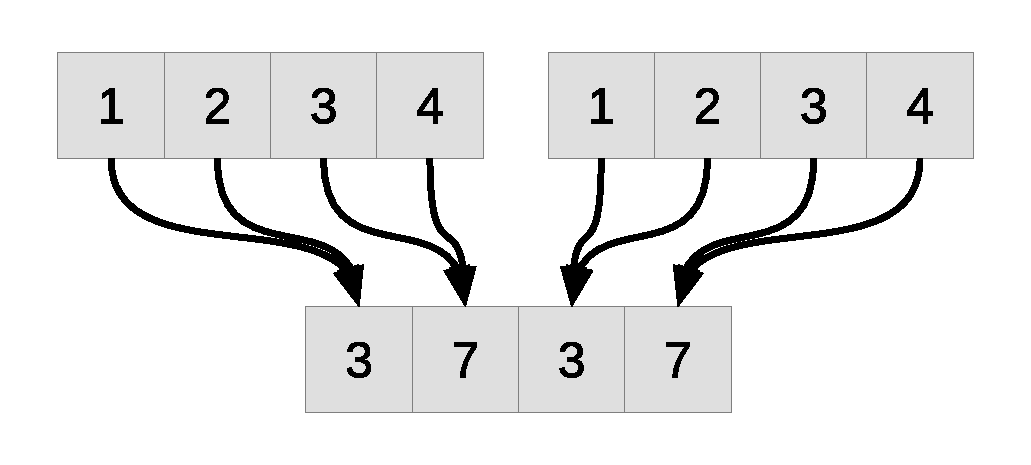
\includegraphics[width=0.5\textwidth]{img/haddps}
\end{center}
\caption{Horizontal Add Packed Single}
\label{fig:haddps}
\end{figure}

The theoretical speed up factor when enriching scalar code with single precision floating point SSE instructions is limited by the maximum number of floats to be processed simultaneously, which is 4. The mentioned vectorization steps constitute a large enough overhead to easily reduce the speed up to a factor of 3. However, this speed up only applies to linear code without control flow statements depending on single data values. Conditional branches (\texttt{if} statements and the like) present a difficult to manage obstacle for SSE optimization that needs to be cleared by using special techniques such as blending. These may sometimes impose a performance drawback that completely consumes the expected vectorization speed ups. In practise, my experiments with SSE and moderately complex code resulted in actual speed up factors between 1.5 and 2 (see section \ref{Evaluation}).

\subsubsection{General techniques for using SSE}
Fortunately, programming with SSE is well supported by modern compilers. Nowadays, there is no need to use inline assembler at all, as Intel, since the very beginning of MMX and SSE, provided so-called specifications for \emph{compiler intrinsics} for C/C++ languages along the SSE specifications. These intrinsics can be used to instruct the compiler to emit a specific SSE instruction, although the compiler is not obliged to actually comply with the programmer's request. For a start, there were two data types defined that help mixing SSE with legacy code: \texttt{\_\_m128} and \texttt{\_\_m128i}. The former maps to a 128 bit wide floating point vector, the latter a 128 bit wide integer vector. These can be seen as additional primitive data types that behave in the fashion of small fixed length arrays of the corresponding type. Recent versions (>= 4.6) of the GNU compiler collection even let the programmer access single elements using the well-known \texttt{[]}-operator. SSE intrinsic names follow consistent patterns: They all start with a \texttt{\_mm\_} prefix, followed by the name of the instruction, followed by the type of the vector's contents. For example, \texttt{\_mm\_hadd\_ps} emits a "Horizontal Add Packed Single" instruction. It takes two \texttt{\_\_m128} arguments and returns another \texttt{\_\_m128} result value. Listing \ref{sse_intrinsics_intro} demonstrates the use of SSE instrinsics for the array sum example given above.
\begin{code}[caption={Array sum using SSE instrinsics}, label=sse_intrinsics_intro]
  __m128 sum = _mm_load_ps(&array[0]);
  for(int i = 4; i < count; i += 4) {
    __m128 add = _mm_load_ps(&array[i]);
    sum = _mm_add_ps(sum, add);
  }

  sum = _mm_hadd_ps(sum, sum);
  sum = _mm_hadd_ps(sum, sum);

  // now sum[0] holds the sum of the floats
\end{code}

The GNU compiler collection recently added support for the usual arithmetic operators for vector types, so instead of writing \texttt{sum = \_mm\_add\_ps(sum, add))} we could also write \texttt{sum += add}. This especially helps to keep readability loss to a minimum. The use of intrinsics has several advantages over inline assembler. First, as mentioned before, the vector types can be treated as if they were primitives. For instance, the programmer does not need to care whether they are stored in registers or in memory. The compiler inserts the appropriate \texttt{mov} instructions when they are needed for calculations. This even includes the possibility to create arrays of vector types. Second and even more important, the use of intrinsics leaves some space for compiler optimization. Whether it be register management or the order of instructions, the compiler may always find ways to further optimize the SSE code. In fact, the compiler may choose not to emit a requested instruction at all, if it sees fit. In a blog entry from 2009~\cite{liranuna2009} the author "LiraNuna" compares the optimized assemblies of the three major SSE-aware compilers. Apart from revealing considerable differences between the produced assemblies, it also displays that all of the popular compilers were able to further optimize simple SSE intrinsics. For example, gcc succeeded in optimizing out 5 useless vector-based arithmetic operations (e.g. multiplying by a vector whose elements are all 1). In sum, there are rarely any situations where inline assembler has any advantages over the use of SSE intrinsics.

Not shown in listing \ref{sse_intrinsics_intro} are the preparations needed for the code to be of actual practical use. Obviously, the array sum would not be correct if count was not a multiple of 4, as then the remaining 1, 2, or 3 elements would not take part in the calculation. There are two options suitable for fixing this issue: Either the programmer could add the remaining elements in a scalar loop right after the vectorized loop (with the iterator starting at the last multiple of 4 less than or equal to count), or he could always pad the array to a length dividable by 4. The padding elements would need to be initialized to zero. Either way would impose a substantial processing overhead (mainly caused by the additional loop) that would render the optimization useless for small arrays. Some other peculiarities of SSE programming are described in the following.

\paragraph{Aligned data storage.} Most SSE instructions that operate on either registers or memory locations require those memory locations to be aligned by 16 byte boundaries (in other words, the memory address needs to be dividable by 16). For instance, \texttt{haddps} allows a memory location as source operand, yet will raise a so-called general protection exception when this location is not aligned by 16 bytes, resulting in an application error. For some SSE instructions such as data move instructions (\texttt{movaps}) there exist instruction variants that allow for unaligned addresses (e.g. \texttt{movups}). However, misaligned addresses still cause long delays and thus should be avoided. Shahbahrami et al. discussed the impact of misaligned accesses in~\cite{shahbahrami2006} [muss ich noch lesen und Stoner auch~\cite{stoner2010}]...


\paragraph{Dealing with conditional branches.} blbalbla


\begin{itemize}
\item aligned vs. unaligned data storage: two ideas: aligned for offset, padding for compound types <-- waste of space, cache?
\item dealing with conditional branches -> branch prediction vs. blending?
\item exploiting NaN values?
\item prefetching \& non-temporal storing -> \texttt{movntps}
\end{itemize}
\subsubsection{New features of SSE4}
\begin{itemize}
\item blendv instead of \texttt{pand}, \texttt{pandn}, \texttt{por}
\item ptest for early exits
\item difficulties when dealing with SSE + AVX?
\end{itemize}
\begin{assembler}
pand   xmm1, xmm0
pandn  xmm0, xmm2
por    xmm0, xmm1
\end{assembler}
\subsection{A word on compiler optimization}
Whenever a programmer chooses to optimize a particular piece of code, he has to be aware of the fact that the compiler - when used with the right set of command line arguments - usually may have already created fairly optimal machine code from that code. As a consequence manual code optimization very often will not yield the desired performance improvements but instead may even slow down the application. Besides, manual optimization will always be a time-consuming task and in the end lead to less readable code. Felix von Leitner gave a striking speech~\cite{leitner2009} about compiler optimization at "Linux Kongress" conference 2009 in which he emphasizes that it is far more important to learn how compiler optimization works and how to structure code in a way that supports compiler optimization than to try to manually outperform the compiler. He concludes that only when the performance boost "drastically" outweighs the decrease in readability, manual optimization really is worth the effort. Again, I would like to point out that the value of manual optimization depends on the very situation. Although on a small scale the compiler will most of the time create fast enough code and manual optimization may not improve performance at all, a human programmer may find optimization measures at a larger scale that speed up execution a lot. The same is true for vectorization: Most modern compilers are able to auto-vectorize specific parts of code such as smaller loops without data dependencies. However, compilers are not able to grasp the complexity of longer loops that could be vectorized as well, for example using branch avoidance techniques as described above.